\documentclass{leaflet}
\usepackage[ngerman]{babel}
\usepackage[utf8]{inputenc} 
\usepackage{blindtext} 
\usepackage{biolinum} 
\renewcommand\rmdefault{\sfdefault}% Verwende serifenlose Schrift 
\usepackage{mwe}% Dummy Bilder 
\usepackage{xcolor} 
\AddToBackground{1}{\put(0,0){\textcolor{blue!20}{\rule{\paperwidth}{\paperheight}}}}%     Farbiger Hintergrund f�r 1. Seite 
\begin{document} 
\title{Veranstalung} 
\author{Veranstalter} 
\date{Veranstaltungstag} 
\maketitle 
\thispagestyle{empty}% Keine Seitenzahlen 
\clearpage 
\section{Willkommen} 
\blindtext 
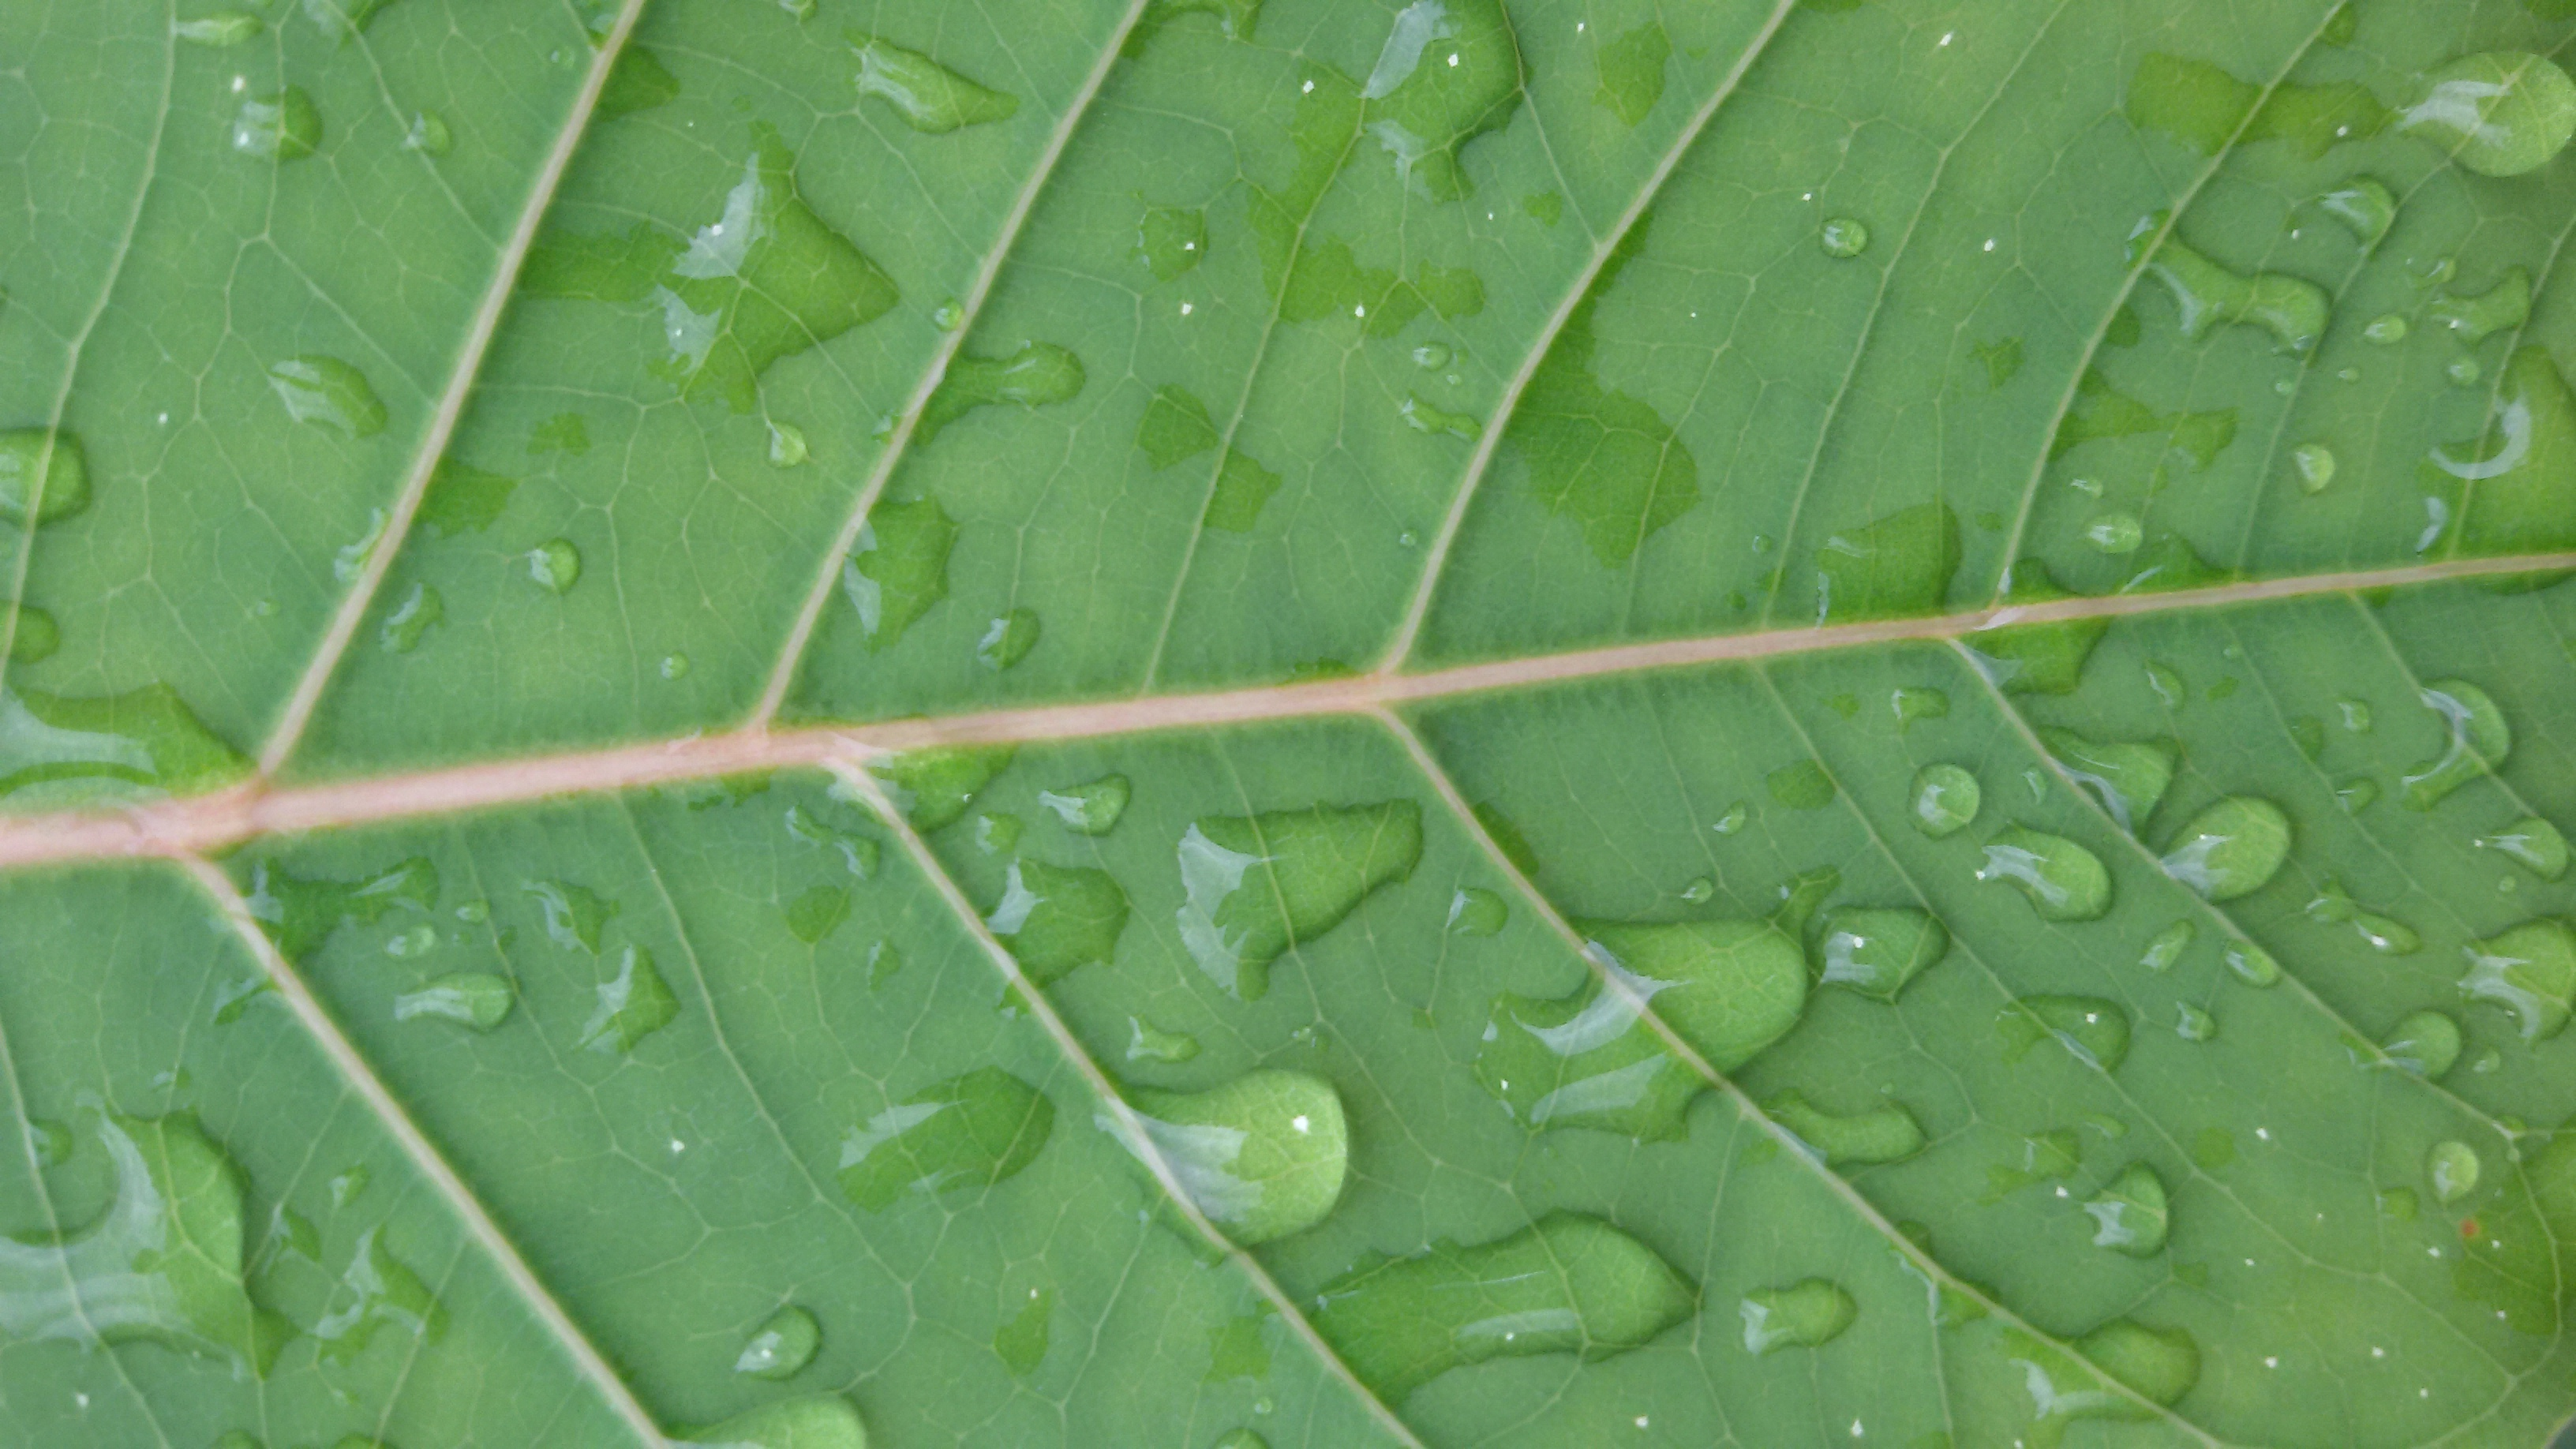
\includegraphics[width=\textwidth]{./example-image-a.jpg}
 \clearpage 
\makebox[\linewidth][l]{\begin{minipage}{2.2\linewidth}
\section{Programm}
 \begin{description} 
\item[Mo.\ 31.03.\ 08:00--16:00] 
\blindtext 
\item[Di.\ 01.04.\ 16:00--19:00] 
\blindtext 
\item[Mi.\ 02.04.\ 10:00--22:00] 
\blindtext \item[Do.\ 03.04.\ 10:00--18:00] 
\blindtext \item[Fr.\ 04.04.\ 10:00--12:00] 
\blindtext 
\end{description}
\end{minipage}}
\clearpage % end the column
\mbox{}
\clearpage % end the spanned column
\section{Danksagung} Ich danke mir! 
\blindtext

\end{document}